% Section 8. Owners: 8.1 Tejas; 8.2 one scenario each (Kushagra, Tejas, Abhishek).
\section{Demonstration of Example System Runs}
\label{sec:demo}

Each scenario runs with one command from a fresh clone (\texttt{make fail-volunteer}, \texttt{make fail-faulty}, \texttt{make fail-leader}). The scripts start a local cluster, inject the failure, keep every log, and print \texttt{PASS} or \texttt{FAIL}.

\subsection{Success Scenario}
\todo{Tejas: one job end to end (TC-01): client progress and the resulting fractal image as screenshots.}

\subsection{Failure Scenario 1: A Volunteer Crashes}
\label{sec:scenario-volunteer}
One coordinator and two volunteers run a job of 256 units, each unit on a single volunteer so that only gossip can rescue a lost unit. Gossip uses a 300\,ms period, a 150\,ms probe timeout and a 2\,s suspect timeout. Once volunteer~A has returned five results, it is killed with \texttt{kill -9}, which gives it no chance to say goodbye. Fig.~\ref{fig:volunteer-crash} shows the terminal output of the run, including the relevant lines of the coordinator log.

\begin{figure*}[t]
\centering
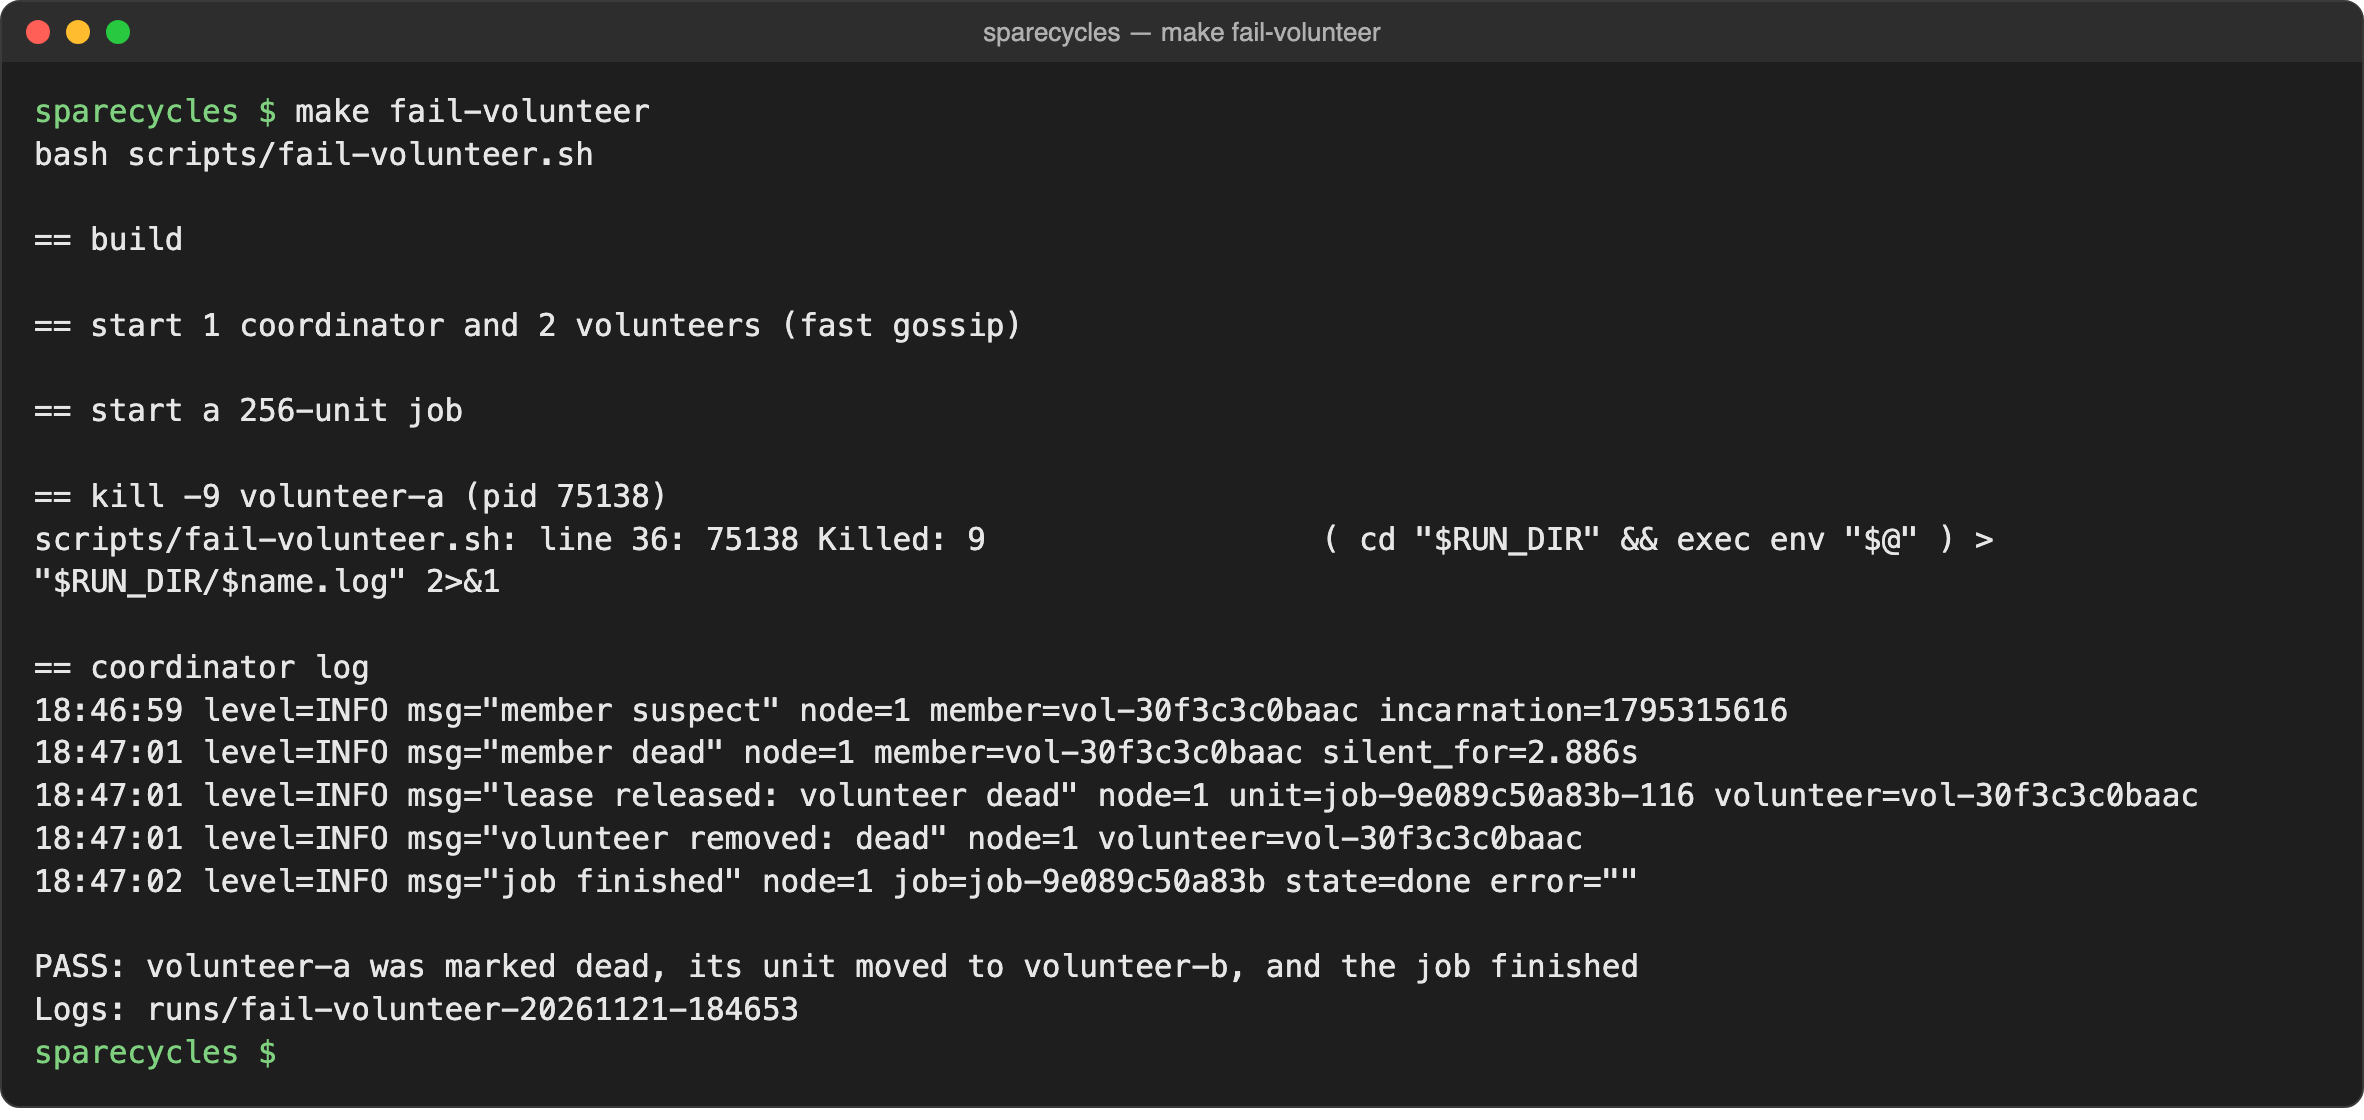
\includegraphics[width=0.9\textwidth]{s2-volunteer-crash.png}
\caption{Terminal output of \texttt{make fail-volunteer}: volunteer~A is killed during a 256-unit job, and the script prints the coordinator log lines for suspicion, death, the released lease and the finished job.}
\label{fig:volunteer-crash}
\end{figure*}

The coordinator first suspected the volunteer at 18:46:59 and declared it dead two seconds later, 2.9\,s after its last contact with it. In the same second it released the lease on unit 116, which volunteer~B then completed, and the job finished one second later. Without gossip the unit would have waited for its full three-minute lease. The volunteer that crashed is also removed from the leader's list; had it been wrongly declared dead, its next request would be refused and it would register again under a new identifier.

\subsection{Failure Scenario 2: A Faulty Volunteer}
\todo{Tejas: after \#7 merges, run \texttt{make fail-faulty} (one volunteer with \texttt{SC\_FAULTY\_RATE=1.0} among three honest ones). Show the \texttt{wrong result} log lines and that the image matches the honest reference.}

\subsection{Failure Scenario 3: The Leader Crashes}
\todo{Abhishek: after \#13 and \#14 merge, run \texttt{make fail-leader}. Show the election, the new term, the table index the new leader continued from, and that the job finished.}
